\let\negmedspace\undefined
\let\negthickspace\undefined
\documentclass[journal,12pt,onecolumn]{IEEEtran}
\usepackage{cite}
\usepackage{amsmath,amssymb,amsfonts,amsthm}
\usepackage{algorithmic}
\usepackage{graphicx}
\graphicspath{{./figs/}}
\usepackage{textcomp}
\usepackage{xcolor}
\usepackage{txfonts}
\usepackage{listings}
\usepackage{enumitem}
\usepackage{mathtools}
\usepackage{gensymb}
\usepackage{comment}
\usepackage{caption}
\usepackage[breaklinks=true]{hyperref}
\usepackage{tkz-euclide} 
\usepackage{listings}
\usepackage{gvv}                                        
\def\inputGnumericTable{}                                 
\usepackage[latin1]{inputenc}     
\usepackage{xparse}
\usepackage{color}                                            
\usepackage{array}                                            
\usepackage{longtable}                                       
\usepackage{calc}                                             
\usepackage{multirow}
\usepackage{multicol}
\usepackage{hhline}                                           
\usepackage{ifthen}                                           
\usepackage{lscape}
\usepackage{tabularx}
\usepackage{array}
\usepackage{float}
\newtheorem{theorem}{Theorem}[section]

\newtheorem{problem}{Problem}
\newtheorem{proposition}{Proposition}[section]
\newtheorem{lemma}{Lemma}[section]
\newtheorem{corollary}[theorem]{Corollary}
\newtheorem{example}{Example}[section]
\newtheorem{definition}[problem]{Definition}

\title{1.3.7}
\author{AI25BTECH11028 -R.Manohar}
\begin{document}
\maketitle
{\let\newpage\relax\maketitle}
\renewcommand{\thefigure}{\theenumi}\renewcommand{\thetable}{\theenumi}
 \bigskip

\textbf{Question}:
\noindent Find the coordinates of the  vertex A of an ABCD parallelogram whose three vertices are given as B$\brak{0,0}$,C$\brak{3,0}$, and D$\brak{0,4}$.
\hfill{(10,2024)}

\textbf{Solution}: From the given information:

\begin{align}
\vec{B} = \myvec{0\\0}, \vec{C} = \myvec{3\\0}, \vec{D} = \myvec{0\\4}
\end{align}

In a paralleleogram,
\begin{align}
\vec{A} = \vec{B} + \vec{D} - \vec{C}\\
= \myvec{0\\0} + \myvec{0\\4} - \myvec{3\\0}\\
= \myvec{-3\\4}
\end{align}
Therefore,Co-ordinates of 
\begin{align}
\vec{A}=\myvec{-3\\4}
\end{align}

From the figure it is clearly verified that the theoretical solution matches with the computational solution.\\
\begin{figure}[h!]
    \centering
    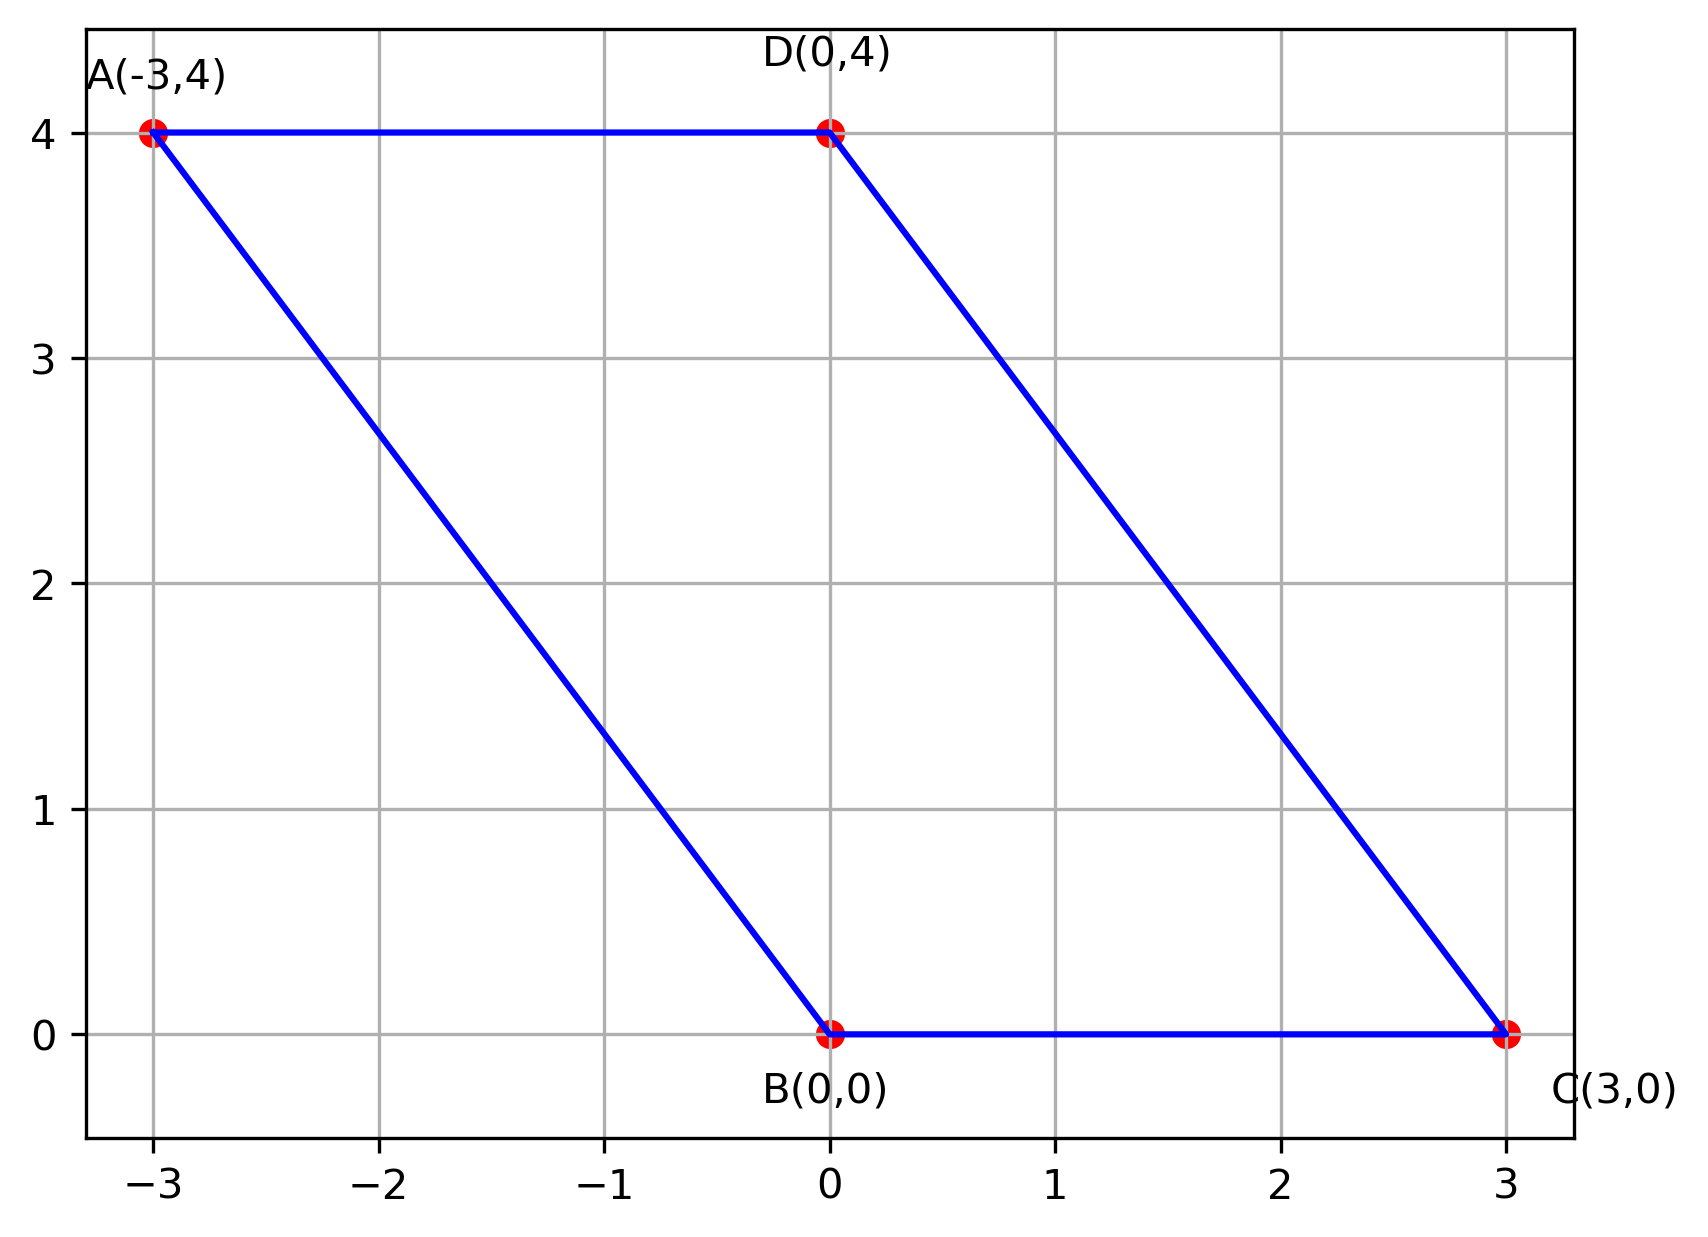
\includegraphics[height=0.5\textheight, keepaspectratio]{figs/figure_1.png}
    \label{figure_1}
\end{figure}






\end{document}